\def\year{2019}\relax
%File: formatting-instruction.tex
\documentclass[letterpaper]{article} %DO NOT CHANGE THIS
\usepackage{aaai19} %Required
\usepackage{times} %Required
\usepackage{helvet} %Required
\usepackage{courier} %Required
\usepackage{url} %Required
\usepackage{graphicx} %Required

\usepackage{thmtools, thm-restate}

\frenchspacing %Required
\usepackage{amsmath,amsthm,amssymb,epigraph,color}
\setlength\epigraphwidth{.8\columnwidth}
\setlength\epigraphrule{0pt}

\setlength{\pdfpagewidth}{8.5in} %Required
\setlength{\pdfpageheight}{11in} %Required
%PDF Info Is Required:
 \pdfinfo{
/Title (Primarily about Primaries)
/Author (Allan Borodin, Omer Lev, Nisarg Shah, Tyrone Strangway)}
\setcounter{secnumdepth}{0} 

% COMMENTS
\newcount\Comments % 0 suppresses notes to selves in text
\Comments = 1
\newcommand{\kibitz}[2]{\ifnum\Comments=1{\color{#1}{#2}}\fi}
\newcommand{\ns}[1]{\kibitz{blue}{[Nisarg: #1]}}
\newcommand{\ab}[1]{\kibitz{red}{[Allan: #1]}}
\newcommand{\ol}[1]{\kibitz{green}{[Omer: #1]}}
\newcommand{\ts}[1]{\kibitz{magenta}{[Tyrone: #1]}}

\newcommand{\citet}[1]{\citeauthor{#1}~\shortcite{#1}}

% THEOREMS
\newtheorem{theorem}{Theorem}
\newtheorem{corollary}[theorem]{Corollary}
\newtheorem{claim}[theorem]{Claim}
\newtheorem{lemma}[theorem]{Lemma}
\newtheorem{proposition}[theorem]{Proposition}
\theoremstyle{definition}
\newtheorem{definition}{Definition}
\newtheorem{example}{Example}
\newtheorem{remark}{Remark}

 % OPERATORS
\newcommand{\upsubset}{\mathbin{\rotatebox[origin=c]{30}{$\subset$}}}
\newcommand{\downsubset}{\mathbin{\rotatebox[origin=c]{-30}{$\subset$}}}
%\DeclarePairedDelimiter{\ceil}{\lceil}{\rceil}
\newcommand{\set}[1]{\left\{#1\right\}}
\renewcommand{\vec}{\overrightarrow}
\renewcommand{\hat}{\widehat}
\renewcommand{\tilde}{\widetilde}
\DeclareMathOperator*{\argmin}{\arg\,\min}
\DeclareMathOperator*{\argmax}{\arg\,\max}

% NOTATION
\newcommand{\bbN}{\mathbb{N}}
\newcommand{\bbR}{\mathbb{R}}
\newcommand{\calI}{\mathcal{I}}
\newcommand{\calM}{\mathcal{M}}
\newcommand{\vsucc}{\vec{\succ}}

% PARTIES
\newcommand{\pleft}{-1}
\newcommand{\pright}{1}
\newcommand{\pind}{0}

% INSTANCES
\newcommand{\all}{\star}
\newcommand{\sep}{\textrm{sep-}}
\newcommand{\euc}[1]{\bbR^{#1}}
\newcommand{\eucsep}[1]{\sep\euc{#1}}
\newcommand{\eucline}{\bbR}
\newcommand{\euclinesep}{\sep\eucline}
\newcommand{\I}{\calI}

% DISTORTION
\newcommand{\dist}{\phi}

% VOTING RULES
\newcommand{\fail}{{\textrm{fail}}}
\newcommand{\maj}{\textrm{maj}}
\newcommand{\plu}{\textrm{plu}}
\newcommand{\borda}{\textrm{Borda}}
\newcommand{\opt}{{\textrm{OPT}}}

 \begin{document}
% The file aaai.sty is the style file for AAAI Press 
% proceedings, working notes, and technical reports.
%
\title{Primarily about Primaries}
\author{Allan Borodin\\University of Toronto\\\texttt{bor@cs.toronto.edu} \And Omer Lev\\Ben-Gurion University\\\texttt{omerlev@bgu.ac.il} \AND Nisarg Shah\\University of Toronto\\\texttt{nisarg@cs.toronto.edu} \And Tyrone Strangway\\University of Toronto\\\texttt{tyrone@cs.toronto.edu}}
\maketitle
\begin{abstract}
Much of the social choice literature examines \emph{direct} voting systems, in which voters submit their ranked preferences over candidates and a voting rule picks a winner. Real-world elections and decision-making processes are often more complex and involve multiple stages. For instance, one popular voting system filters candidates through \emph{primaries}: first, voters affiliated with each political party vote over candidates of their own party and the voting rule picks a candidate from each party, which then compete in a general election. 

We present a model to analyze such multi-stage elections, and conduct the first quantitative comparison (to the best of our knowledge) of the direct and primary voting systems with two political parties in terms of the quality of the elected candidate. Our main result is that every voting rule is guaranteed to perform almost as well 
(i.e., within a constant factor) under the primary system as under the direct system. Surprisingly, the converse does not hold: we show settings in which there exist voting rules that perform significantly better under the primary system than under the direct system.
\end{abstract}

\section{Introduction}

\epigraph{\emph{If I could not go to heaven but with a party, I would not go there at all.}}{-- Thomas Jefferson, 1789}

Thomas Jefferson, like many of the US constitution's authors, believed that political parties and factions are a bad thing (see also \citet{HMJ87}). This view stemmed from a long history of British and English political history, in which prison sentences and executions were possible outcomes in the battle between factions for supremacy at the Royal court~\cite{Sim07}. However, both in Britain and in the Unites States, once their respective legislative assemblies gained political force, parties turned out to be quite unavoidable. Even Jefferson had to start his own party, which ended up quite successful, and was able to vanquish the opposing party from political existence~\cite{Wil05}.

Fast forwarding to today, political parties have become the bedrock of parliamentary politics throughout the world. In particular, one of political parties' main roles -- if not the most important (especially in presidential systems) -- is to select the candidates which are voted for by the general public. The mechanisms by which parties make this selection are varied, and they have evolved significantly throughout the past 150 years. But in the past few decades there has been a marked shift by parties throughout the world towards increasing the ability of individual party (or unaffiliated) members to influence the outcome, and in some cases, to be the only element to determine party candidates~\cite{CB11}. In particular, US parties have changed their election methods since the 1970s to focus the selection of presidential, congressional and state-wide candidates on popular support by party members via primaries~\cite{CKNZ08}.

Despite this long and established role of parties in whittling down the candidate field in elections, the treatment of a parties' role in elections within the multiagent systems community has been quite limited. While various candidate manipulation attacks have been investigated (e.g., Sybil attacks~\cite{CM10}), and there is recent research into parties as a collection of similar minded candidates (e.g., in gerrymandering, across different districts), the role of parties in removing candidates has not been explored.

%In this paper we have two goals. The first, to set out a {\bf model} of multi-stage elections, which can encompass a wide variety of settings. In particular, it can model systems in which only a small subset selects the candidate (e.g., the old system in British parties), a system in which party members elect them (primaries), or a range of other options, which include multiple stages. Our model is based on single-peaked preferences in multi-dimensional space (which allows for any set of preferences to be modeled), and therefore allows for considerations of each candidate's utility to each voter, allowing for comparisons with the outcomes of different voting rules.

%Our second goal is to further investigate {\bf pure primary systems}, in which parties' entire electorate selects from among each party's candidates, and then the general public selects the ultimate election winner. In particular, we examine the difference between such systems and direct elections (i.e., without primaries), and examine the \emph{distortion} level of each election method. We show that, in the worst case, primary systems cannot have much worse distortion than direct elections, while they can improve upon them in some cases.

%\ns{Check from here.} 
The focus of this paper is the \emph{primary} voting system, in which each party's electorate selects a winner from among the party's candidates, and among these primary winners, an ultimate election winner is selected by the general public. Our goal is to compare this system to the \emph{direct} voting system, in which all voters directly vote over all candidates. 

\subsection{Our Results} 
Our contribution is twofold. First, we formulate a model which allows a quantitative comparison of the two voting systems. Our model is a spatial model of voting in which voters and candidates lie in an underlying multi-dimensional space, and voter preferences are single-peaked. This allows us to compare each candidate's social utility in terms of its total distance to the voters. We make the evaluation metric formal using the notion of \emph{distortion} advocated by a recent line of research~\cite{PR06,BCHL+15}. Our results focus on 2 parties, each selecting a single candidate, with both candidates presented to the general voting public.

Second, we use this model to present a comparison of the direct and primary voting systems. In particular, we show that no voting rule performs much worse (by more than a constant factor) under the primary system than under the direct system. While the converse holds in some cases, we show settings in which it does not, and there exist voting rules that perform much better under the primary system than under the direct system.% \ns{To here.}

It is important to note that while we write of parties, voters and elections, this multi-step model applies to a variety of decision-making processes by agents. An organization selecting an ``employee of the month'' may ask each unit to nominate a single candidate, and then choose from amongst them. A city may ask its regional subdivisions to assess which roads require urgent fixing, and then the city council decides from these options where to invest its efforts. Fundamentally, in many cases where the potential number of options is huge, it is common to use subdivisions to cull the options and present only a few of them for discussion and vote. In such cases, our multi-stage model is apt. %ns - Should be in discussion

\section{Related Work}

The analysis of regular, direct elections is long and varied, both in the social sciences and in AI~\cite{BCELP16}. In our particular setting, the voters are located in a metric space, with their preferences related to their distance from candidates. Such settings have been widely investigated in the social science literature since the work of \citet{Dow57}, recently summarized by \citet{Sch08}. In particular, we focus on the idea of distortion in such elections, a topic broached by \citet{PR06} for voters with a utility function, but investigated in the context of voters in metric spaces in a series of papers~\cite{ABP15,AP17,SE17} for most common voting rules. \citet{FFG16} explored such a setting for strategyproof mechanisms.

Discussing changes to the set of candidates has been mainly focused on two paths of research. Strategic candidates, investigation of which began with the work of \citet{DJL01} -- followed by \citet{DJL02} discussing strategic candidacy in tournaments, and recently further explored by \citet{BC15}, \citet{PORKJ15} and others -- deals mainly with finding equilibria. The other is the addition and removal of candidates, as a form of control manipulation, which was studied by \citet{BTT92}; see the summaries by \citet{BCELP16} and \citet{Rot15}.

Investigating parties' selection methods and their effect on the election has mostly been done in the social sciences. \citet{Ken09} details the range of selection methods parties use, and there has been significant focus on more democratic methods for leader selection~\cite{CK13}, which seems to be a general trend in many Western countries~\cite{CB11}. There is also significant literature on particular party elections in various countries, such as Britain \cite{JW10}, Belgium \cite{Wau10}, Israel \cite{Haz97}, and many others. Naturally, the most widely examined country is the US, in which political parties have been a fixture of political life since its early days \cite{Wil05}. The most recent extensive summary of research on it is due to \citet{CKNZ08}, who try to explain how party power-brokers influence the party membership vote. \citet{Nor04} uses primary data to predict election results, and notably \citet{STVW18} show that primary voters are very similar to ``regular'' voters. In computational fields, recent interest in proxy voting~\cite{CMMMO17,KMP18}, in which voters give other agents the ability to vote for them, may be related to how modern parties are viewed and analyzed.

\section{Model}
\label{sec:model}

For $k \in \bbN$, define $[k] = \set{1,\ldots,k}$. Let $V = [n]$ denote a set of $n$ \emph{voters}, and $A$ denote a set of $m$ \emph{candidates}. We assume that voters and candidates lie in an underlying metric space $M = (S,d)$, where $S$ is a set of points and $d$ is a distance function satisfying the triangle inequality and symmetry. More precisely, there exists an \emph{embedding} $\rho : V \cup A \to S$ mapping each voter and candidate to a point in $S$. For a set $X \subseteq V \cup A$, we slightly abuse the notation and let $\rho(X) = \set{\rho(x) : x \in X}$. Also, for $x,x' \in V \cup A$, we often use $d(x,x')$ instead of $d(\rho(x),\rho(x'))$ for notational convenience.

In this work, we assume that voters and candidates additionally have an affiliation with a political party. Specifically, we study a setting with two parties\footnote{The model can be extended to multiple parties in a reasonably straightforward manner, but for simplicity's sake, we shall focus on only 2 parties.}, denoted $\pleft$ and $\pright$. The \emph{party affiliation} function $\pi : V \cup A \to \set{\pleft,\pright}$ maps each voter and candidate to the party they are affiliated with. For $p \in \set{\pleft,\pright}$, let $V_p = \pi^{-1}(p) \cap V$, $A_p = \pi^{-1}(p) \cap A$, $n_p = |V_p|$, and $m_p = |A_p|$. We require $n_p \ge 1$ for each $p \in \set{\pleft,\pright}$. Our main result (Theorem~\ref{thm:large-primaries-good}) holds even if there are independent voters not affiliated with either party. %independent voters that participate in the general election but not in the primaries), and we have pushed to the appendix showing that allowing only of a fraction of the voters to participate in the general election only increases the distortion by a fixed multiple.
%ns - This doesn't affect our results (just makes the analysis simpler) because we have an unbounded number of voters. So we can always add one voter in the other party in a way that doesn't affect anything by much. 

%ns : We don't impose $n_p, m_p \ge 1$ for each $p \in \set{\pleft,\pright}$ so some of our results are easier.

Collectively, an \emph{instance} is the tuple $I = (V,A,M,\rho,\pi)$. Given $I$, our goal is to find a candidate $a \in A$ as the winner. The \emph{social cost} of $a$ is its total distance to the voters, denoted $C^I(a) = \sum_{i \in V} d(i,a)$. For party $p \in \set{\pleft,\pright}$, let $C^I_p(a) = \sum_{i \in V_p} d(i,a)$. Hence $C^I(a) = C^I_{\pleft}(a) + C^I_{\pright}(a)$. We also use for $X \subseteq V$, $C^I_X(a) = \sum_{i \in X} d(i,a)$. Given an instance $I$, we would like to choose a candidate $a_{\opt} \in \argmin_{a \in A} C^I(a)$ that minimizes the social cost. We shall drop the instance from superscripts if it is clear from the context.

However, we do not observe the full instance. Specifically, we do not know the underlying metric $M$ or the embedding function $\rho$. Instead, each voter $i \in N$ submits a a \emph{vote}, which is a ranking (strict total order) $\succ_i$ over the candidates in $A$ by their distance to the voter. Specifically, for all $i \in N$ and $a,b \in A$, $a \succ_i b \Rightarrow d(i,a) \le d(i,b)$. The voter is allowed to break ties between equidistant candidates arbitrarily. The \emph{vote profile} $\vsucc^I = (\succ_1,\ldots,\succ_n)$ is the collection of votes. Given an instance $I$, its corresponding \emph{election} $E^I = (V,A,\vsucc^I,\pi)$ contains all observable information. 

In the families of instances that we consider, we fix the number of candidates $m$ and let the number of voters $n$ to be arbitrarily large. This choice is justified because in many typical elections (e.g., political ones), voters significantly outnumber candidates. Let $\calI^{\alpha}_{m,\calM}$ be the family of instances satisfying the following conditions.
\begin{itemize}
	\item Each party has at least an $\alpha$ fraction of the voters affiliated with it, i.e., $n_p \ge \alpha \cdot n$ for each $p \in \set{\pleft,\pright}$. Note that $\alpha \in [0,0.5]$: $\alpha = 0.5$ is the strictest (exactly half of the voters are affiliated with each party), while $\alpha=0$ imposes no conditions; in the latter case, we omit the superscript $\alpha$. 
	\item The number of candidates is at most $m$.%\footnote{For common voting rules, the distortion is typically an increasing function of $m$, and this condition is equivalent to the number of candidates being equal to $m$. However, we need it to be at most $m$ for some of our results to apply to \emph{all} voting rules.}
	\end{itemize}
	In particular, we shall focus on a few cases of $\calM:$
\begin{description}
	\item[$\calM=\star$] This allows $M$ to be an arbitrary metric space. 
	\item[$\calM = \bbR^k$] The metric space should be $M = (\bbR^k,d)$, where $d$ is the standard Euclidean distance.
	\item [$\calM = \textrm{sep-}\bbR^k$] This means the embedding $\rho$ must be such that $\rho(V_{\pleft} \cup A_{\pleft})$ and $\rho(V_{\pright} \cup A_{\pright})$ are linearly separable.\footnote{Two sets of points are linearly separable if the interiors of their convex hulls are disjoint, or equivalently, if there exists a hyperplane that contains each set in a distinct closed halfspace.} In this case we shall take the metric to be $M = (\bbR^k,d)$ with $d$ as the standard Euclidean distance. In plain words, the voters and candidates affiliated with each party reside in a certain part of the metric space, separate from those affiliated with the other party. In a single dimension, this means there exists a threshold on the line such that voters and candidates affiliated with one party lie to the left of it, while those affiliated with the other party lie to the right. %That is, there is a set of parameters which is shared between all party members and candidates (and not shared with the other party). For example, in a single dimensional space, a left-right split.
	Note that this is the only choice of $\calM$ that restricts the embedding $\rho$ based on party affiliation $\pi$. 
\end{description}

These families of instances are related by the following relation. For all $k$, 
$$
\I^{\alpha}_{m,\eucsep{k}} \ \ 
\substack{\upsubset \\[0.1cm] \downsubset} \ \ 
\substack{\I^{\alpha}_{m,\euc{k}} \\[0.5cm] \I^{\alpha}_{m,\eucsep{k+1}}} \ \ 
\substack{\downsubset \\[0.1cm] \upsubset} \ \ 
\I^{\alpha}_{m,\euc{k+1}} \subset \I^{\alpha}_{m,\all}
$$

\subsection{Voting Rules and Distortion}

A voting rule $f$ takes an election as input, and returns a winning candidate from $A$. We say that the cost-approximation of $f$ on instance $I$ is 
$$
\phi(f,I) = \frac{C^I(f(E^I))}{\min_{a \in A} C^I(a)},
$$
and given a family of instances $\calI$, the distortion of $f$ with respect to $\calI$ is
$$
\phi_{\calI}(f) = \sup_{I \in \calI} \phi(f,I).
$$


Since distortion is a worst-case notion, we have that when $\calI \subseteq \calI'$, $\phi_{\calI}(f) \le \phi_{\calI'}(f)$ for every voting rule $f$.

Standard voting rules choose the winning candidate independently of party affiliations. These include rules such as plurality, Borda count, $k$-approval, veto, and STV. We refer readers to the book by \citet{BCELP16} for their definitions. We call a voting rule \emph{affiliation-independent} if $f(E) = f(E')$ when elections $E$ and $E'$ differ only in their party affiliation functions. Since an affiliation-independent voting rule $f$ ignores party affiliations, we have $\phi_{\I^{\alpha}_{m,\eucsep{k}}}(f) = \phi_{\I^{\alpha}_{m,\euc{k}}}(f)$. All of the above-mentioned rules, in addition to being affiliation-independent, share the property of being \emph{unanimous}, i.e., they return candidate $a$ when $a$ is the top choice of all voters.

\subsection{Stages and Primaries}
%In most cases, political parties often do not allow the general electorate to consider the full set of their candidates. Instead, they conduct an internal selection process, at the end of which they select a set of candidates (or a single one) to run in the election. This process may have multiple stages, but the common system, employed in the main US, Canadian and other countries' parties is one of primaries, in which party members vote on the set of their party's candidates in one stage. We focus on this system.

Given an affiliation-independent voting rule $f$, voting systems with primaries employ a specific process to choose the winner, essentially resulting in a different voting rule $\hat{f}$ that operates on a given election $E = (V,A,\vsucc,\pi)$ as follows:
\begin{enumerate}
	\item First, it creates two \emph{primary elections}: for $p \in \set{\pleft,\pright}$, define $E_p = (V_p,A_p,\vsucc_p,\pi_p)$, where $\vsucc_p$ denotes the preferences of voters in $V_p$ over candidates in $A_p$, and $\pi_p : V_p \to \set{p}$ is a constant function. 
	\item Next, it computes the winning candidate in each primary election (primary winner) using rule $f$: for $p \in \set{\pleft,\pright}$, let $a^*_p = f(E_p)$.
	\item Finally, let $E_g = (V,\set{a^*_{\pleft},a^*_{\pright}},\vsucc_g,\pi)$ be the \emph{general election}, where $\vsucc_g$ denotes the preferences of all voters over the two primary winners. The winning candidate is $\hat{f}(E) = \maj(E_g)$, which is what most voting rules become when dealing with only 2 candidates.\footnote{If one of the parties has no affiliated candidates, then the primary winner of the other party becomes the overall winner. In a setting with more than 2 parties, or where each party nominates several candidates, the general election can use $f$ to determine the outcome (or use some other voting process).} Here, $\maj$ is the majority rule, which, given two candidates, picks the one that a majority of voters prefer; our results are independent of its tie-breaking. 
\end{enumerate}
This resembles systems employed by the main US, Canadian and other countries' parties, in which a party's members vote on their party's candidates to select a winner of their primary. In other systems, such selection could be a multi-stage process.

Given an affiliation-independent voting rule $f$, the goal of this paper is to compare its performance under the \emph{direct system}, in which $f$ is applied on the given election directly, to its performance under the \emph{primary system}, in which $\hat{f}$ is applied on the given election instead. Formally, given a family of instances $\calI$ and an affiliation-independent voting rule $f$, we wish to compare $\phi_{\calI}(f)$ and $\phi_{\calI}(\hat{f})$ (henceforth, the distortion of $f$ with respect to $\calI$ under the direct and the primary systems, respectively). 

\section{Small Primaries Are Terrible}
\label{sec:small-primaries}

Recall that in a family of instances $\I_{m,\calM}^{\alpha}$, we require that at least $\alpha$ fraction of voters be affiliated with each party, i.e., $n_p \ge \alpha n$ for each $p \in \set{\pleft,\pright}$. In other words, each primary election must have at least $\alpha n$ voters. 

We first show that when a primary election can have very few voters ($\alpha = 0$), every reasonable voting rule has an unbounded distortion in the primary system, even with respect to our most stringent family of instances $\I_{m,\euclinesep}$. 
\begin{theorem}
	For $m \ge 3$, $\phi_{\I_{m,\euclinesep}}(\hat{f}) = \infty$ for every affiliation-independent unanimous voting rule $f$.
\label{thm:small-primaries-bad}
\end{theorem}
\begin{proof}
	Consider an instance $I \in \I_{m,\euclinesep}$ in which voter $1$ is located at $0$ and affiliated with party $\pleft$, while the remaining $n-1$ voters are located at $1$ and affiliated with party $\pright$. All $m$ candidates are affiliated with party $\pleft$: one is at $0$, and the rest are at $1$.
	
	The candidate $a^*$ at $0$ becomes the primary winner of party $\pleft$, and trivially becomes the overall winner. Its social cost is $C(a^*) = n-1$. In contrast, an optimal candidate $a_{OPT}$ at $1$ has social cost $C(a_{OPT}) = 1$. Hence, $\frac{C(a^*)}{C(a_{OPT})} = n-1$. Since the number of voters $n$ is unbounded, $\phi_{\I_{m,\euclinesep}}(\hat{f}) = \infty$.
\end{proof}

Theorem~\ref{thm:small-primaries-bad} continues to hold even if we require that at least a constant fraction of candidates be affiliated with each party: we could simply move a constant fraction of the candidates from $1$ to $3$, and the proof would still go through. 

On the other hand, if we require that at least a \emph{constant fraction of voters} be affiliated with each party, the result changes dramatically.

\section{Large Primaries Are Never Much Worse}
\label{sec:large-primaries-good}

For every affiliation-independent voting rule $f$, we bound the distortion of $\hat{f}$ in terms of the distortion of $f$ \emph{for every instance}. Note that this is stronger than comparing the worst-case distortions of $f$ and $\hat{f}$ over a family of instances.

Given an instance $I = (V,A,M,\rho,\pi)$ and party $p \in \set{\pleft,\pright}$, we say that $I_p = (V_p,A_p,M,\rho_p,\pi_p)$ is the \emph{primary instance} of party $p$, where $\rho_p$ and $\pi_p$ are restrictions of $\rho$ and $\pi$ to $V_p \cup A_p$. The primary election $E_p$ of party $p$ is precisely the election corresponding to instance $I_p$. 

%We are now ready to state the main result of this paper. To present the result in its most general form, we allow a subset of voters $V_g \subseteq V$ to participate in the general election under the primary system. Our result shows that the winner under the primary system has low social cost as long as at least a constant fraction of voters --- split arbitrarily between $V_{\pleft}$ and $V_{\pright}$ --- vote in the general election. 

\begin{theorem}
	Let $I = (V,A,M,\rho,\pi)$ be an instance. For $p \in \set{\pleft,\pright}$, let $I_p$ be the primary instance of party $p$, and $n_p = |V_p| \ge \alpha n$. Then,
	$$
	\phi(\hat{f},I) \le 3 \cdot \frac{1-\alpha+\max(\phi(f,I_{\pleft}),\phi(f,I_{\pright}))}{\alpha}.
	$$
	Further, for a socially optimal candidate $a_{OPT} \in \argmin_{a \in A} C^I(a)$, we have a bound depending only on the distortion of the primary election of its party:
	$$
	\phi(\hat{f},I) \le 3 \cdot \frac{1-\alpha+\phi(f,I_{\pi(a_{OPT})})}{\alpha}.
	$$

\label{thm:large-primaries-good}
\end{theorem}

For each family of instances $\I$ that we study, it holds that for every instance $I \in \calI$, both its primary instances, if seen as direct elections, are also in $\I$ (since the party division has no effect on the direct election distorition). Hence, we can convert the instance-wise comparison to a worst-case comparison. 

\begin{corollary}
\label{cor:large-primaries-good}
	For every $\alpha > 0$, $k \in \bbN$, family of instances $\I \in \set{\I_{m,\all},\I_{m,\euc{k}},\I_{m,\eucsep{k}}}$, and affiliation-independent voting rule $f$, 
	$$
	\phi_{\I}(\hat{f}) \le 3\cdot \frac{1-\alpha+\phi_{\I}(f)}{\alpha}.
	$$ 
\end{corollary}

Note that $\phi_{\I}(f) \ge 1$ by definition. Hence, we can write $\phi_{\I}(\hat{f}) \le \frac{6}{\alpha} \cdot \phi_{\I}(f)$. In other words, for every affiliation-independent voting rule $f$, its distortion under the primary system is at most a constant times bigger than its distortion under the direct system, with respect to every family of instances that we consider. %Moreover, both Theorem~\ref{thm:large-primaries-good} and Corollary~\ref{cor:large-primaries-good} hold when the different parties are using different voting rules, when using the $f$ with the higher distortion value.

%
%Theorem~\ref{thm:large-primaries-good} is slightly stronger, though. Even if we use a voting method whose distortion --- recall that distortion is measured in the worst case over inputs --- may be bad, it will perform well under the primary system as long as the two primary elections are not bad instances for that voting method. We now turn to proving this result. First, we need two useful lemmas.

To prove Theorem~\ref{thm:large-primaries-good}, we need two lemmas. The first lemma shows that if the distortion of a rule $f$ for a primary instance $I_p$ is low, then the corresponding primary winner $a^*_p$ is nearly as good as any candidate in $A_p$ for the overall election as well. The intuition is that when voters in $V \setminus V_p$ drive up the social cost of $a^*_p$ (i.e., when they are far from $a^*$), they must do so for every candidate in $A_p$. 

\begin{lemma}
\label{lem:winner-opt-same-party}
	Let $a^*_p$ denote the primary winner of party $p$. Then 
	$$
	C(a^*_p) \le \frac{1-\alpha+\phi(f,I_p)}{\alpha} \cdot \min_{a \in A_p} C(a).
	$$
\end{lemma}
\begin{proof}
	Let $\theta = \phi(f,I_p)$ (hence $\theta\geq 1$). Fix an arbitrary $a \in A_p$. Then, $C_{V_p}(a^*_p) \le \theta \cdot C_{V_p}(a)$. %We want $C(a^*_p) \le (1-\alpha+\beta)/\alpha \cdot C(a)$, where $C$ is the overall social cost. 
	Now, 
	\begin{align}
	C(a^*_p) &= C_{V_p}(a^*_p) + C_{V\setminus V_{p}}(a^*_p) \nonumber\\
	&\le \theta\cdot C_{V_p}(a) + C_{V\setminus V_{p}}(a) +(n-n_{p}) \cdot d(a,a^*_p) \nonumber\\
	&\le \theta \cdot C(a) + (n-n_{p}) \cdot d(a^*_p,a),
	\label{eqn:lem1-eq1}
	\end{align}
	where the second transition follows %because $C_{V\setminus V_{p}}(a^*_p) \le C_{V\setminus V_{p}}(a) + (n-n_{p}) \cdot d(a^*_p,a)$ 
	due to the triangle inequality. 
	%ns - This is where we can't allow independent voters.
	We also have $d(a^*_p,a) \le d(a^*_p,i)+d(i,a)$ for any $i \in V_p$. Thus, 
	\begin{align}
	d(a^*_p,a) &\le \frac{C_{V_p}(a^*_p)+C_{V_p}(a)}{n_p} \nonumber\\
	&\le \frac{1+\theta}{n_p} \cdot C_{V_p}(a) \le \frac{1+\theta}{n_p} \cdot C(a).
	\label{eqn:lem1-eq2}
	\end{align}
	
	Substituting Equation~\eqref{eqn:lem1-eq2} into Equation~\eqref{eqn:lem1-eq1}, and using the fact that $\frac{n-n_{p}}{n_p} \le \frac{1-\alpha}{\alpha}$, we get the desired result. 
\end{proof}

Our next lemma shows that the primary winner that wins the general election is not much worse than the primary winner that loses the general election. 
\begin{lemma}
\label{lem:winners-two-parties}
	Let $a^*_{\pleft}$ and $a^*_{\pright}$ be the two primary winners, $a^* \in \set{a^*_{\pleft},a^*_{\pright}}$ be the winner of the general election, and $\hat{a} \in \set{a^*_{\pleft},a^*_{\pright}} \setminus \set{a^*}$. Then, 
	$$
	C(a^*) \le 3 \cdot C(\hat{a}).
	$$
\end{lemma}
\begin{proof}
Because $a^*$ wins the general election by a majority vote, there must exist $X \subseteq V$, $|X| \ge \frac{n}{2}$ such that $d(i,a^*) \le d(i,\hat{a})$ for every $i \in X$. Combining with the triangle inequality $d(a^*,\hat{a}) \le d(a^*,i) + d(i,\hat{a})$, we get $d(i,\hat{a}) \ge \frac{d(a^*,\hat{a})}{2}$ for every $i \in X$. Hence,
\small
	\begin{equation}
	C(\hat{a}) \ge \frac{n}{2} \cdot \frac{d(a^*,\hat{a})}{2} \Rightarrow d(a^*,\hat{a}) \le \frac{4}{n} \cdot C(\hat{a}).
	\label{eqn:lem2-eq1}
	\end{equation}
\normalsize
	Now, we have
	\small
	\begin{align}
	C(a^*) &= \sum_{i \in X} d(i,a^*) + \sum_{i \in V \setminus X} d(i,a^*) \nonumber\\
	&\le \sum_{i \in X} d(i,\hat{a}) + \sum_{i \in V \setminus X} (d(i,\hat{a}) + d(a^*,\hat{a})) \nonumber\\
	&\le C(\hat{a}) + \frac{n}{2} \cdot d(a^*,\hat{a}),
	\label{eqn:lem2-eq2}
	\end{align}
	\normalsize
	where the second transition follows because $d(i,a^*) \le d(i,\hat{a})$ for $i \in X$, and $d(i,a^*) \le d(i,\hat{a})+d(a^*,\hat{a})$ due to the triangle inequality. Substituting Equation~\eqref{eqn:lem2-eq1} into Equation~\eqref{eqn:lem2-eq2}, we get the desired result. 	
\end{proof}

We are now ready to prove our main result.

\begin{proof}[Proof of Theorem~\ref{thm:large-primaries-good}]
	Recall that $a^*_{\pleft}$ and $a^*_{\pright}$ are the primary winners. Let $p \in \set{\pleft,\pright}$ be such that $a^*_p$ is the winner of the general election. Let $a_{OPT} \in \argmin_{a \in A} C(a)$ be a socially optimal candidate. We consider three cases.
	
	\begin{itemize}
		\item \emph{Case 1: $a_{OPT} \in A_p$.} That is, the optimal candidate and the winner are affiliated with the same party. In this case, Lemma~\ref{lem:winner-opt-same-party} yields 
		$$
		\phi(\hat{f},I) \le \frac{1-\alpha + \phi(f,I_p)}{\alpha}=\frac{1-\alpha + \phi(f,I_{\pi(a_{OPT})})}{\alpha}.
		$$
		 
		\item \emph{Case 2: $a_{OPT} \in A_{-p}$, $a_{OPT} = a^*_{-p}$.} That is, the optimal candidate and the winner are affiliated with different parties, and the optimal candidate is a primary winner. In this case, Lemma~\ref{lem:winners-two-parties} yields 
		$$
		\phi(\hat{f},I) \le 3.
		$$
		
		\item \emph{Case 3: $a_{OPT} \in A_{-p}$, $a_{OPT} \neq a^*_{-p}$.} That is, the optimal candidate is affiliated with a party different than that of the winner, and is not a primary winner. In this case, we use both Lemmas~\ref{lem:winner-opt-same-party} and~\ref{lem:winners-two-parties} to derive
		\small
		\begin{align*}
		\phi(\hat{f},I) &= \frac{C(a^*_p)}{C(a_{OPT})} = \frac{C(a^*_p)}{C(a^*_{-p})} \cdot \frac{C(a^*_{-p})}{C(a_{OPT})} \\
		&\le 3 \cdot \frac{1-\alpha+\phi(f,I_{-p})}{\alpha} \\
		&=3 \cdot \frac{1-\alpha+\phi(f,I_{\pi(a_{OPT})})}{\alpha}.
		\end{align*}
		\normalsize
	\end{itemize}
	Thus, in each case, we have the desired approximation.
\end{proof}

Note that our proof of Theorem~\ref{thm:large-primaries-good} does not preclude the existence of \emph{independent voters}. Specifically, we can allow the party affiliation function $\pi$ to map a subset of voters $V_0$ to a neutral choice (say $0$), have these voters only vote in the general election and not in either primary election under the primary system, and the proof of Theorem~\ref{thm:large-primaries-good} would still go through. Additionally, we can also relax the restriction that all voters vote in the general election. That is, we can assume that a subset of voters $V_g \subseteq V$ vote in the general election under the primary system, assume $|V_g| \ge \gamma n$, and a version of Theorem~\ref{thm:large-primaries-good} in which the constant $3$ in the bound is replaced by $\frac{4-\gamma}{\gamma}$ would hold. This requires a generalization of Lemma~\ref{lem:winners-two-parties}, omitted due to space constraints. Finally, notice that we do not use the assumption that both parties use the same voting rule $f$ in their primaries. The theorem extends easily to allow the use of different voting rules, with the distortion under the primary system still being bounded in terms of the maximum of the distortions in the two primary elections. 

\section{Large Primaries Are Not Better\\Without Party Separability}
\label{sec:large-primaries-not-better-all}

While we showed in the previous section that a voting rule does not perform much worse under the primary system than under the direct system, we now show that it does not perform any better either, at least in the worst case over all instances with at most $m$ candidates. The result continues to hold even if we require each party to have at least a constant fraction of the voters. 

Note that this result is weaker than Theorem~\ref{thm:large-primaries-good} because it is a worst-case comparison instead of an instance-wise comparison. However, it still applies to all voting rules $f$. It applies to any metric that does not require separability of parties, in particular to $\I_{m,\all}$ and $\I_{m,\euc{k}}$.

\begin{theorem}
\label{thm:large-primaries-not-better-all}
	For $\alpha \in [0,0.5]$, $k \in \bbN$, $\calM \in \set{\star,\bbR^k}$ (i.e. when the metric space does not require party separability), and affiliation-independent voting rule $f$, we have $\phi_{\I^{\alpha}_{m,\calM}}(\hat{f}) \ge \phi_{\I^{\alpha}_{m,\calM}}(f)$. 
\end{theorem}
\begin{proof}
We shall denote $\I^{\alpha}_{m,\calM}$ as $\I$. We want to show that for every instance $I \in \I$, there exists an instance $I' \in \I$ such that $\phi(\hat{f},I') \ge \phi(f,I)$. This would imply the desired result.
	
	Fix an instance $I = (V,A,M,\rho,\pi) \in \I$. Let $a_{OPT} \in A$ denote an optimal candidate in $I$, and $a^* = f(E^I)$. Note that $\phi(f,I) = \frac{C^I(a^*)}{C^I(a_{OPT})}$. Construct instance $I' = (V',A,M,\rho',\pi')$ as follows. 
	\begin{itemize}
		\item Let $V' = V \cup \tilde{V}$, where $\tilde{V}$ is a new set of voters and $|\tilde{V}| = |V|$.
		
		\item Let $\rho'(x) = \rho(x)$ for all $x \in V \cup A$, and $\rho(x) = \rho(a_{OPT})$ for all $x \in \tilde{V}$. That is, $\rho'$ matches $\rho$ for existing voters and candidates, and the new voters are co-located with $a_{OPT}$.
		
		\item Let $\pi'(x) = \pleft$ for all $x \in V \cup A$, and $\pi'(x) = \pright$ for all $x \in \tilde{V}$. That is, all existing voters and candidates are affiliated with party $\pleft$, while all new voters are affiliated with party $\pright$.
	\end{itemize}

	First, let us check that $I' \in \I$. Since $I$ has $m$ candidates, so does $I'$. Further, in $I'$, we have $|V'_{\pleft}| = |V'_{\pright}| = |V'|/2$, which satisfies the constraint corresponding to every $\alpha \in [0,0.5]$. Hence, we have $I' \in \I$. 

	Let us apply $\hat{f}$ on $I'$. One of its primary instances, $I'_{\pleft}$, is precisely $I$. Hence, the primary winner of party $\pleft$ is $f(I'_{\pleft}) = f(I) = a^*$. Because there are no candidates affiliated with party $\pright$, $a^*$ becomes the overall winner.\footnote{Even if we require each party to have at least one affiliated candidate, the proof essentially continues to hold. In this case, we can add one candidate affiliated with party $\pright$ that is located sufficiently far from all the voters, ensuring that $a^*$ still becomes the overall winner. This would show $\phi_{\I^{\alpha}_{m+1,\calM}}(\hat{f}) \ge \phi_{\I^{\alpha}_{m,\calM}}(f)$ because instance $I'$ may now have $m+1$ candidates.}
	
	Next, $C^{I'}(a^*) \ge C^I(a^*)$ because $V \subset V'$. Also, $C^{I'}(a_{OPT}) = C^I(a_{OPT})$ because $a_{OPT}$ has zero distance to all voters in $V' \setminus V$. Together, they yield 
	\begin{equation}
	\phi(\hat{f},I') = \frac{C^{I'}(a^*)}{C^{I'}(a_{OPT})} \ge \frac{C^I(a^*)}{C^I(a_{OPT})} = \phi(f,I),
	\label{eqn:translate-worst-case}
	\end{equation}
	as desired.
% OLD PROOF. KEEPING IT AROUND IN CASE THERE IS A BUG IN THE NEW ONE.	
%	Consider a worst-case instance for the direct system with $n/2$ voters and $m-1$ in which voters and candidates are embedded into a metric space $M$, candidate $\hat{a}$ is the winner, but there exists candidate $a^*$ such that $C(\hat{a}) = \beta \cdot C(a^*)$. 
%	
%	Let us construct an instance of the primary system with the same voting method. Let the aforementioned worst-case instance be the primary election corresponding to party $L$. Let $V_R$ consist of $n/2$ new voters located exactly where $a^*$ is located, and $A_R$ consist of a single candidate $\overline{a}$ that is sufficiently far from all other candidates and all voters. Then, $\hat{a}$ still wins the primary election corresponding to party $L$, and $\overline{a}$ wins the primary election corresponding to party $R$ due to lack of competition. Since $\overline{a}$ is sufficiently far, all voters vote for $\hat{a}$ in the general election, making $\hat{a}$ the overall winner. 
%	
%	Let $\overline{C}$ denote the social cost function in the new primary instance. Then, $\overline{C}(\hat{a}) \ge C(\hat{a})$, while $\overline{C}(a^*) = C(a^*)$ because the additional $n/2$ voters contribute no cost to $a^*$. Hence, $\overline{C}(\hat{a}) \ge \beta \cdot \overline{C}(a^*)$, i.e., $\distprim^\metall(f) \ge \beta$, as required.
\end{proof}

Our proof actually establishes a slightly stronger result. Instead of showing $\phi_{\I^{\alpha}_{m,\calM}}(\hat{f}) \ge \phi_{\I^{\alpha}_{m,\calM}}(f)$, we actually show $\phi_{\I^{0.5}_{m,\calM}}(\hat{f}) \ge \phi_{\I^{\alpha}_{m,\calM}}(f)$. 

\section{Separability and Its Advantages}
\label{sec:large-primaries-better-line}

The analysis for $\I_{m,\eucsep{k}}$ is not so straightforward. In the proof of Theorem~\ref{thm:large-primaries-not-better-all}, we co-located the new voters affiliated with party $\pright$ and $a_{OPT}$ affiliated with party $\pleft$. This was allowed because non-separable metrics like $\all$ and $\euc{k}$ place no constraints on the embedding. 

With $\I^{\alpha}_{m,\eucsep{k}}$, we need the voters and candidates affiliated with one party to be separated from those affiliated with the other. Hence, this operation of putting all of one party's voters at the location of $a_{OPT}$ belonging to another party would be allowed only if, in the original instance $I$, $a_{OPT}$ is on the boundary of the convex hull of $\rho(V \cup A)$. While this is not the case for all instances, we only need this in at least one \emph{worst-case instance} for $f$, i.e., for at least one $I \in \I^{\alpha}_{m,\eucsep{k}}$ with $\phi(f,I) = \phi_{\I^{\alpha}_{m,\eucsep{k}}}(f)$. Equation~\eqref{eqn:translate-worst-case} would then yield the desired result. More generally, it is sufficient if, given any $\epsilon > 0$, we can find an instance $I$ such that $\phi(f,I) \ge \phi_{\I^{\alpha}_{m,\eucsep{k}}}(f) - \epsilon$ and $a_{OPT}$ is at distance at most $\epsilon$ from the boundary of the convex hull of $\rho(V \cup A)$. 

%$$
%\phi_{\I^{\alpha}_{m,\eucsep{k}}}(\hat{f}) \ge \phi(\hat{f},I') \ge \phi(f,I) = \phi_{\I^{\alpha}_{m,\eucsep{k}}}(f).
%$$ 

Interestingly, \cite{ABP15} show that this is indeed the case for plurality and Borda count (see the proof of their Theorem 4). Thus, we have the following.

\begin{proposition}
	Let $f$ be plurality or Borda count. Then, $\phi_{\I^{0.5}_{m,\euclinesep}}(\hat{f}) \ge \phi_{\I_{m,\all}}(f)$.
\label{prop:plu-borda}
\end{proposition}

%
%\begin{definition}
%	We say that an affiliation-independent voting rule $f$ has an \emph{extreme worst case} if there exists an instance $I = (V,A,M,\rho,\pi) \in \I_{m,\euclinesep}$ such that $\phi(f,I) = \phi_{\I_{m,\all}}(f)$ and for an optimal candidate $a_{OPT} \in \argmin_{a \in A} C^I(a)$, either $\rho(a_{OPT}) \le \rho(x)$ for all $x \in V \cup A$ or $\rho(a_{OPT}) \ge \rho(x)$ for all $x \in V \cup A$.
%\end{definition}
%
%\begin{theorem}
%	For an affiliation-independent voting rule $f$ that has an extreme worst case, $\phi_{\I^{0.5}_{m,\euclinesep}}(\hat{f}) \ge \phi_{\I_{m,\all}}(f)$.
%\end{theorem}
%
%Note that due to the definition of distortion, the result holds if we replace $\I^{0.5}_{m,\euclinesep}$ on the left hand side with any family that is a superset, and replace $\I_{m,\all}$ on the right hand side with any family that is a subset. 
%
%\citet[Proof of Theorem 4]{ABP15} show that plurality and Borda count have an extreme worst case by explicitly constructing such a worst case instance. Thus, we have the following.
%
%\begin{proposition}
%	Plurality and Borda count have an extreme worst case.
%\end{proposition}

However, known worst cases for the Copeland rule~\cite{ABP15} and STV~\cite{SE17} do not satisfy this requirement. It is unknown if these rules admit a different worst case that satisfies it. 

This raises an important question. \emph{Does Proposition~\ref{prop:plu-borda} hold for all affiliation-independent voting rules?} We shall shortly answer this \emph{negatively}.

More precisely, we construct an affiliation-independent voting rule $f$ such that $\phi_{\I^{\alpha}_{m,\euclinesep}}(\hat{f}) \ll \phi_{\I^{\alpha}_{m,\euclinesep}}(f)$ for every $\alpha > 0$. That is, with large primaries, $f$ performs much better under the primary system than under the direct system, when voters and candidates are embedded on a line and the separability condition is imposed. 

Note that instances in $\I_{m,\euclinesep}$ are highly structured. For instance, it is known that when voters and candidates are embedded on a line, there always exists a weak Condorcet winner~\cite{Bla48}, and selecting such a candidate results in a distortion of at most $3$~\cite{ABP15}. Hence, we have $\phi_{\I_{m,\euclinesep}}(f) = 3$ for every Condorcet-consistent, affiliation-independent voting rule $f$.\footnote{\cite{ABP15} also proved that no affiliation-independent (deterministic) voting rule can have distortion better than $3$, even with respect to $\I_{m,\euclinesep}$.}

Our aim in this section is to construct an affiliation-independent voting rule $f_\fail$ that with respect to $\I_{m,\euclinesep}$ has an unbounded distortion in the direct system, but at most a constant distortion in the primary system.% In particular, we need the argument laid out at the end of the previous section --- which led to Proposition~\ref{prop:plu-borda} --- to fail for $f_\fail$. For this, we need to ensure that in every instance that is a worst case for $f_\fail$ with respect to $\I_{m,\euclinesep}$, an optimal candidate should be sufficiently far from both endpoints. The challenge is that we are not given any cardinal information about distances in the underlying metric. Given only ranked preferences, can we detect if a certain candidate is sufficiently far from both endpoints? Surprisingly, we answer this positively.

\begin{definition}
	Let $f_\fail$ be an affiliation-independent voting rule that operates on election $E = (V,A,\vsucc)$ as follows. Let $A = \set{a_1,\ldots,a_m}$, and $t = (m+1)/2$. 
\begin{itemize}
	\item \emph{Special Case}: If $m \ge 9$, $m$ is odd, $n \ge m^2$, and $\vsucc$ has the following structure, then return $a_1$.
	\begin{enumerate}
		\item For voter $1$, $a_1 \succ_1 \ldots \succ_1 a_m$.
		\item For voter $2$, $a_m \succ_2 \ldots \succ_2 a_1$.
		\item For voter $3$, $a_{t-1}$ is the most preferred, and \\ $a_{m-2} \succ_3 a_1 \succ_3 a_{m-1} \succ_3 a_m$.
		\item For voter $4$, $a_{t+1}$ is the most preferred, and \\ $a_3 \succ_4 a_m \succ_4 a_2 \succ_4 a_1$.
		\item For $j \in [m-2]$, for voter $i = 4+(2j-1)$, \\ $a_{j+1} \succ_i a_{j+2} \succ_i a_j$, and for voter $i' = 4+2j$, \\ $a_{j+1} \succ_{i'} a_j \succ_{i'} a_{j+2}$.
		\item For every other voter $v$, $a_t$ is the most preferred.
			\end{enumerate}
	
	\item If $E$ does not fall under the special case, then apply any Condorcet consistent voting rule (e.g., Copeland's rule).
\end{itemize}
\end{definition}
\begin{figure*}
\centering
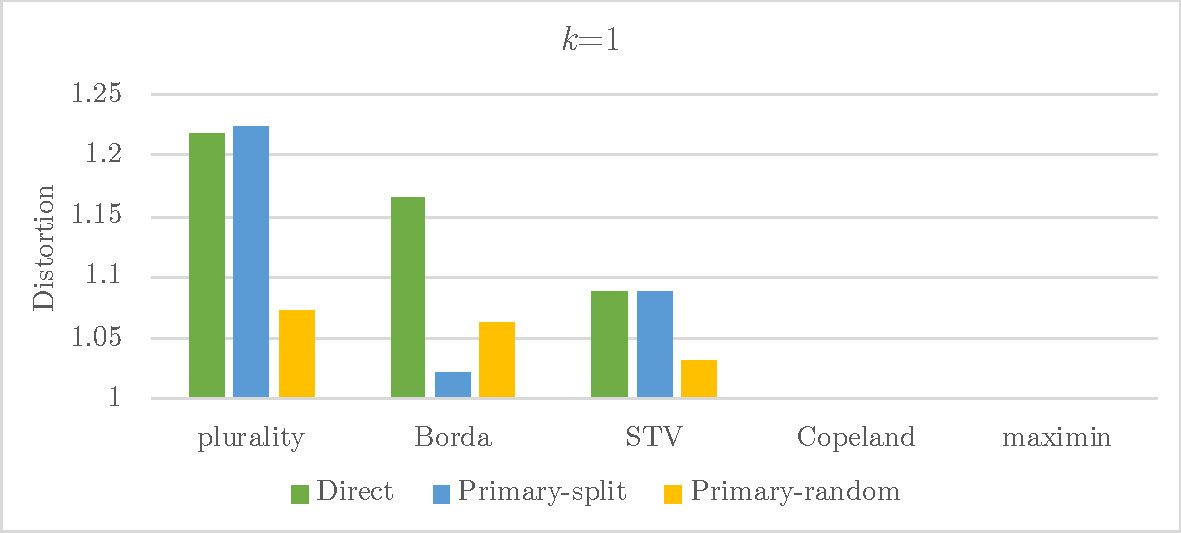
\includegraphics[width=0.47\linewidth]{distortion_1.pdf}
\hspace{0.05\linewidth}
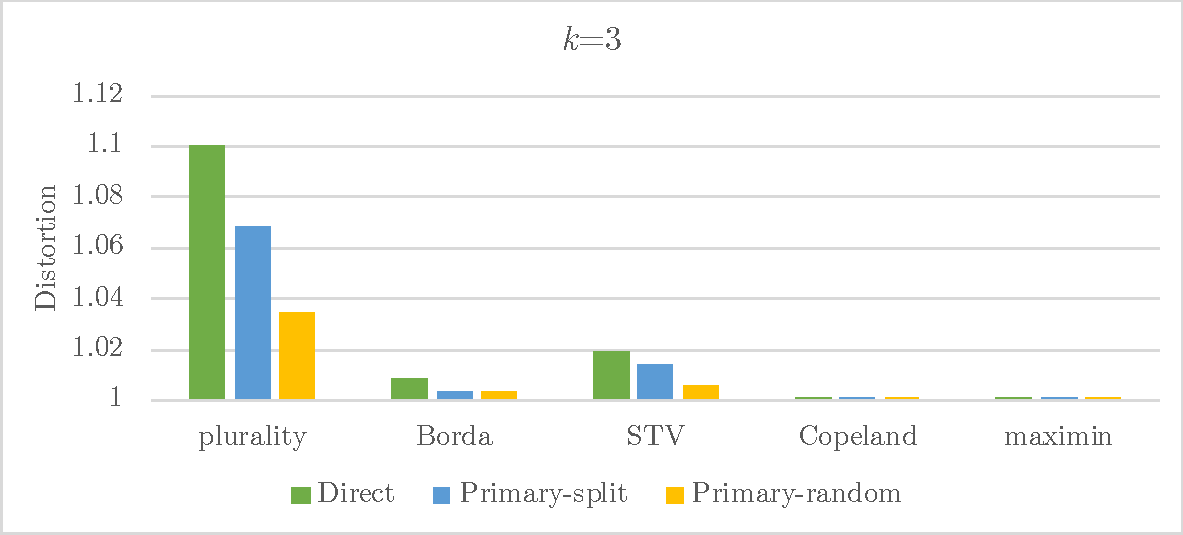
\includegraphics[width=0.47\linewidth]{distortion_3.pdf}
\caption {The distortion values for various settings (Direct, Primary-split and Primary-random) and voting rules for $k \in \set{1,3}$. Each bar represents the average distortion over $1000$ instances. Within each figure, all of the bars represent average distortion over the same set of voter and candidate locations, but not necessarily party affiliations. ANOVA on all elections returned $p<10^{-9}$ when $k=1$ and $p<10^{-5}$ when $k=3$}
\label{distortions}
\end{figure*}

Note that $m$ being odd ensures that $t$ is an integer, and $m \ge 9$ ensures that $a_1$, $a_3$, $a_{t-1}$, $a_t$, $a_{t+1}$, $a_{m-2}$, and $a_m$ are all distinct candidates. The significance of $n \ge m^2$ will be clear later. 

We will now establish that a worst-case instance of $f_\fail$ falls under the special case; for this instance, we need to show that $a_t$ is socially optimal; that $f_\fail$ returns $a_1$ on this instance; and most importantly, that the structure of $\vsucc$ ensures that the optimal candidate $a_t$ is sufficiently far from both the leftmost and the rightmost candidates. 

We prove this last fact in the following lemma. 

\begin{lemma}
	Let $I = (V,A,M,\rho,\pi) \in \I_{m,\euclinesep}$ be an instance for which the corresponding election $E^I$ falls under the special case of $f_\fail$. Then the following holds.
	\begin{enumerate}
		\item Either $\rho(a_1)\leq\ldots\leq\rho(a_{m})$, or $\rho(a_{1})\geq\ldots\geq\rho(a_{m})$, or $|\rho(A)|=2$.%, with $\rho(v_{1})=\rho(v_{2})=sgn(x_{2}-x_{1})\frac{x_{2}-x_{1}}{2}$.
		\item If $|\rho(A)|\neq 2$, %or $|\rho(A)|=2$ and $\rho(a_{1})= \rho(a_{m})$, 
		$min\set{d(a_t,a_1),d(a_t,a_m)} \ge \frac{d(a_1,a_m)}{4}$.
	\end{enumerate}
	\label{lem:special-clause}
\end{lemma}

The proof of the lemma, and the proof of the next theorem is omitted due to space constraints.

\begin{theorem}
	For $m \ge 9$ and constant $\alpha \in (0,0.5]$, $\phi_{\I^{\alpha}_{m,\euclinesep}}(\hat{f}_\fail)$ is upper bounded by a constant, whereas $\phi_{\I^{\alpha}_{m,\euclinesep}}(f_\fail)$ is unbounded.
	\label{thm:primary-much-better}
\end{theorem}

\section{Using Simulations to Go Beyond Worst Case}

So far we compared the distortion of a voting rule under the direct and primary systems, taken in the \emph{worst case} over a family of instances. In practice, such worst case instances may not arise naturally. In this section, we compare the distortion of a voting rule under the direct and primary systems, in the \emph{average case} over simulated instances. To control for the effect of vastly different numbers of voters or candidates affiliated with the two parties, we place the restriction that half of the voters and half of the candidates must be affiliated with each party. Furthermore, we wish to examine instances in which voters and candidates affiliated with one party are separated from those affiliated with the other party. 

We fix the metric space to be $[0,1]^k$ for $k \in \set{1,3,5,7,9}$ with the Euclidean distance. We generate $1000$ instances satisfying the following restrictions. First, we place a set $V$ of $n = 1000$ voters at uniformly random locations in $[0,1]^k$. Next, we find a hyperplane dividing voters into two equal halves. Due to symmetry, we simply find a threshold $t$ on the $k^{\text{th}}$ coordinate such that the locations of half of the voters (call this set $V_{\pleft}$) have a smaller $k^{\text{th}}$ coordinate, while the locations of the rest (call this set $V_{\pright}$) have a greater $k^{\text{th}}$ coordinate. We do not affiliate the voters yet. Next, we place $\frac{m}{2} = 10$ candidates (call this set $A_{\pleft}$) uniformly at random on one side of the hyperplane,  and $\frac{m}{2} = 10$ candidates (call this set $A_{\pright}$) uniformly at random on the other side.

Once the locations of the voters and candidates are fixed, we create two instances. In one instance (``split''), we assign $V_{\pleft} \cup A_{\pleft}$ to party $\pleft$, and assign $V_{\pright} \cup A_{\pright}$ to party $\pright$. This instance belongs to $\I^{0.5}_{m,\eucsep{k}}$. In the other instance (``random''), we assign half of the voters and half of the candidates chosen uniformly at random to party $\pleft$, and the rest to party $\pright$. This instance belongs to $\I^{0.5}_{m,\euc{k}}$, but not necessarily to $\I^{0.5}_{m,\eucsep{k}}$. This allows us to directly compare the effect that separability has on the distortion. Finally, we run five voting rules --- plurality, Borda, STV, Copeland and maximin --- on both instances under the direct and primary systems, and measure the distortion. Note that their distortion under the direct system would be identical for both instances because the two instances only differ in party affiliations. Thus, for each rule, we obtain three numbers: Direct, Primary-split, and Primary-random. We average the distortion numbers across the $1000$ instances. 

See Figure~\ref{distortions} for selected simulation results. The results for $k > 3$ resemble those for $k=3$ in their comparison of the direct versus the primary system; the only difference is that the overall distortions are lower for higher $k$. To compare the three distortion numbers in each case, we ran a repeated measures ANOVA comparing the distortion values, and in all but 2 of 25 cases, had a $p$ value under $0.05$ (the two cases had $k=9$). 

Perhaps the most important observation is that our simulation results stand in direct contrast to our worst-case bounds. In almost all of our settings, the distortion under the primary system (split and random) is better than that the distortion under its direct counterpart, and often shows a significant improvement. This is especially noticeable in the non-Condorcet consistent rules (plurality, Borda and STV), as in all but 3 of 15 cases the distortion significantly improves the primary system in both cases. This effect is most pronounced with plurality. With Condorcet consistent rules, the distortion values are very low, regardless of whether the direct system is used or the primary system. In general, as we increase the dimension $k$, the groups become more homogenous and the $p$ values grow, while distortions  approach $1$.

Overall, the simulation results show a distortion that is far below our theoretical worse-case results. We suspect that the reason for this difference might have to do with our choice of uniform voter and candidate distributions, and distortion numbers might differ under different distributions.

\section{Discussion}

%In this paper we explored the topic of multi-stage elections, in which, prior to the general elections, a subset of voters can decide which candidates will continue to the next stage. In particular, we focus on the 2-stage primary model, used in various party systems throughout the world, in which parties vote on who their leader shall be, and subsequently these parties' leaders contest the general election.

%Using this model we show primary elections cannot produce significantly worse results than direct elections. In addition, for many natural voting rules we also find that primary systems  might produce a worst case distortion which is about the same as in the direct system. However, we are able to construct a voting rule and setting in which the primary system has an unbounded advantage (again in the worst case) over the corresponding direct system.  All in all, our theoretical results show primaries can in some instances improve the election system's distortion, and they cannot hurt the distortion too much.

Our paper initiates the novel quantitative study of multi-stage elections (and their comparison to single-stage elections), but leaves plenty to explore. Some directions are fairly straightforward extensions of our results. The most straightforward question is to tighten our bounds. There is also the question of explaining the trends we observe in the average case, which sometimes differ from our worst-case results. A next step would be to study realistic distributional models of voter preferences and candidate positions in the political spectrum, and analyze their effect on distortion.
 
Other extensions are seemingly more involved. Extending our framework to more than two parties requires the use of a ranked voting rule in the general election, which may significantly affect the analysis. Interestingly, such an extension would also incorporate independent candidates because one can imagine an independent candidate to be a party of their own. Examining the use of multiple and different voting rules as \citet{NW13} do for two-step voting (though without candidate elimination between stages) is an enticing direction. For example, in a multi-party direct system, we may use plurality, whereas in the primary system, the parties may use STV. It is also reasonable to consider that each party has its own voting rule. It would be interesting as well to examine party manipulation techniques in primary systems. Similarly, it is reasonable to believe that candidates may also strategically shift, to some extent, their location following the primaries, to make themselves more appealing to the general electorate. 

We believe that the study of multi-stage elections and party mechanisms can not only contribute novel theoretical challenges to tackle, but can also bring research on computational social choice closer to reality and increase its impact. 

\section{Acknowledgements}
This work was partially supported by NSERC under the Discovery Grants program.
%References and End of Paper
%These lines must be placed at the end of your paper
\small
\bibliographystyle{aaai}
\bibliography{abb,general}

\end{document}
